\section{WebPosTransaction.java Class}
The performed \emph{Code Inspection} activity has been focused on the \emph{WebPosTransaction.java} class. That class is related to the \textit{webpos} package which contains a plugin tha may be integrated with other functionalities provided by \textit{OFBiz} in order to provide to the user functionalities related to the management of a web POS: a browser based Point of Sale solution.

The complete source path of the class in the release \emph{16.11.01} of the \emph{Apache OFBiz project} is:\\

\centerline{\tt apache-ofbiz-16.11.01/specialpurpose/webpos/src/main/java/}
\centerline{\tt /org/apache/ofbiz/webpos/transaction/WebPosTransaction.java} \hfill

The class is located in the package:\\
\centerline{\tt org.apache.ofbiz.webpos.transaction}

\subsection{The \textit{webpos} package}
The webpos package java suource code related to a plugin that may be integrated with the \emph{Apache OFBiz} suite of applications.

It is composed by three main subpackage and a Java class:
\begin{itemize}
	\item \texttt{org.apache.ofbiz.webpos.}\textbf{search} package\\Contains a java class to manage some searching functionalities (for example about facilities and products).
	\item \texttt{org.apache.ofbiz.webpos.}\textbf{session} package\\Contains a java class representing a web pos session.
	\item \texttt{org.apache.ofbiz.webpos.}\textbf{transaction} package\\Contains a java class representing  a single web pos transaction.
	\item \texttt{org.apache.ofbiz.webpos.}\textbf{WebPosEvents.java} class\\Java class to manage incoming requests from the related web based application.
\end{itemize}

\subsection{Functional Role of the Class}
The \emph{WebPosTransaction.java} class doesn't have any form of documentation or \emph{Javadoc} (\url{https://ci.apache.org/projects/ofbiz/site/javadocs}) making really hard the comprehension of its functionalities from a source code analysis.

For these reasons we will provide an high-level overview of the functionality role of the class in relation with related java classes. The description provided is based upon our interpretation of the source code, some documentation about other classes of the project and UML class diagrams generated from the code, so it may not correspond entirely to a right description of the intention of the java class author.\\

The \emph{WebPosTransaction.java} class identifies a single transaction in the context of a \emph{WebPosSession}. The transaction is also related to a \emph{ShoppingCart} object, hold by the session, and its methods allow to manage the payment procedure also instantiating the order related to the cart checkout. \\

In \autoref{fig:package} are shown relations between components in the \emph{webpos} package with respect to the \emph{WebPosTransaction.java} class:
\begin{itemize}
	\item Te \emph{WebPosEvents} class has a method \emph{completeSale} that after obtaining the current transaction through the \emph{getCurrentTransaction} method (exposed by the \emph{WebPosSession}) interacts with it calling the \emph{processSale} method\todo{ref sotto}
	\item 
\end{itemize}

\begin{figure}[h]
			\centering
			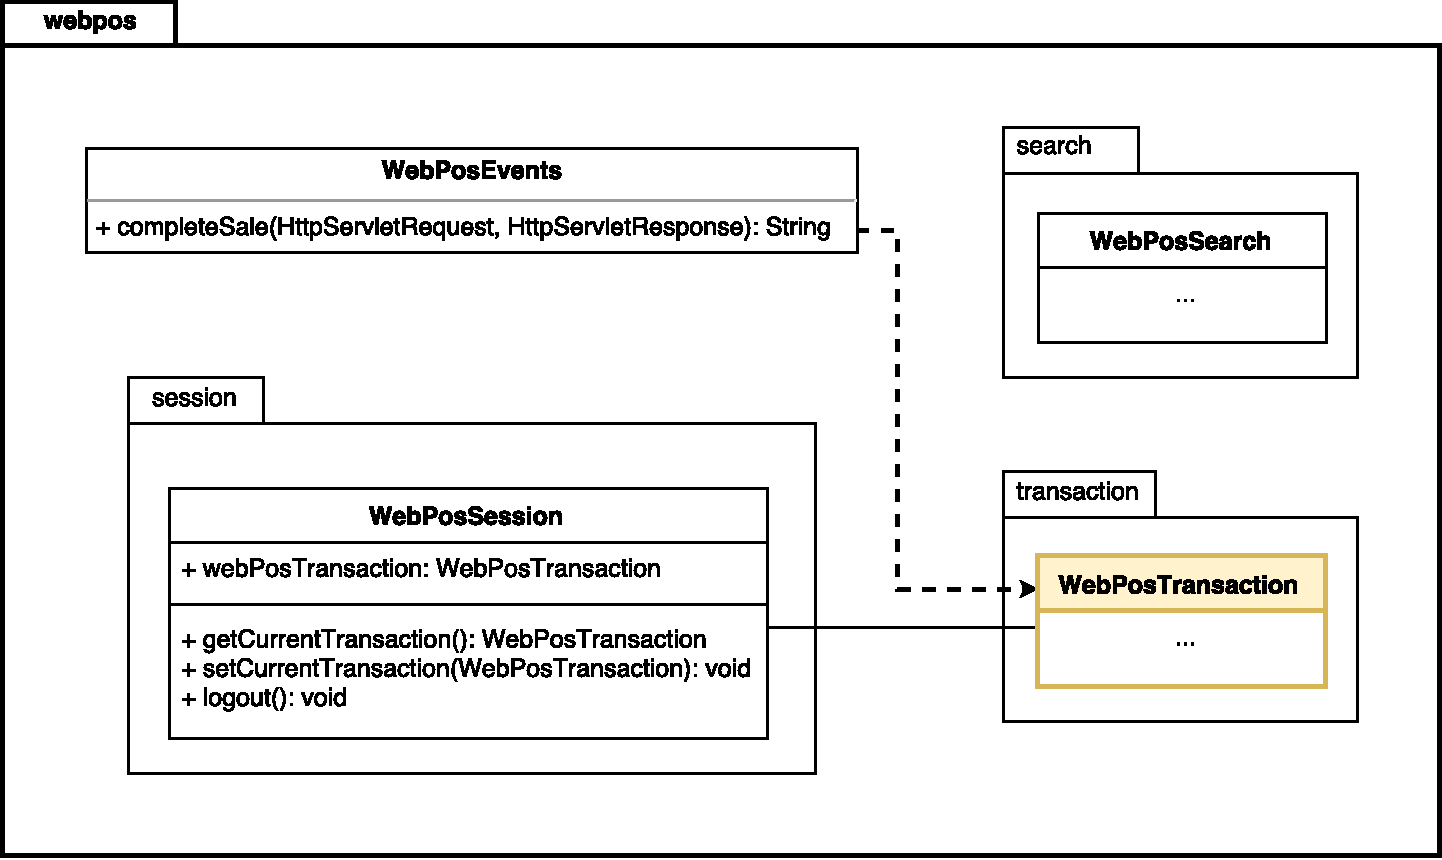
\includegraphics[scale=0.4]{package}
			\caption{
				\label{fig:package} 
				\emph{WebPosTransaction.java} relations inside the \emph{webpos} package
			}
		\end{figure}

\subsection{Class Description}
The class contains the logic to manage a transaction but the specified methods are supposed to be called from an higher level component holding the transaction object.

\subsubsection{Fields}
The main fields of the class (excluding constant \emph{final static} fields)  are \emph{private} fields:

\begin{itemize}
    \item \textbf{CheckOutHelper ch} instance of \\ \texttt{org.apache.ofbiz.order.shoppingcart.CheckOutHelper}: an object that provides functionalities to manage the cart related to the order in the checkout phase.
    \item \textbf{GenericValue txLog} instance of \\ \texttt{org.apache.ofbiz.entity.GenericValue}: persistent entity identifying a \emph{PosTerminalLog}, a logger where are stored logs about the transaction
    \item \textbf{String transactionId}: a string to store the identifier of the transaction
    \item \textbf{String orderId}: a string to store the identifier of the order related to the transaction
    \item \textbf{String partyId}: a string to store the identifier of the party
    \item \textbf{boolean isOpen}: a boolean value, set as \emph{true} if there exist a \emph{PosTerminalState} opened
    \item \textbf{int drawerIdx} (field not used in the current implementation of the class, the related getter always return 1)
    \item \textbf{GenericValue shipAddress} instance of \\ \texttt{org.apache.ofbiz.entity.GenericValue}: persistent entity identifying the \emph{PostalAddress} entity related to the shipping address
    \item \textbf{WebPosSession webPosSession} instance of \\ \texttt{org.apache.ofbiz.entity.GenericValue}: the current session managing the transaction
\end{itemize}

\paragraph{Notes} Some notes about concepts used inside the \emph{OFBiz} project:
\begin{itemize}
 	\item An Entity is a relational data construct that contains any number of Fields and can be related to other entities \cite{OFBiz}. Entities are managed by the \emph{entity engine} to be used from java classes transparently from their actual implementation.
\end{itemize}

\subsubsection{Methods}

The main methods of the class (excluding getter methods and methods which functionalities are based upon a unique call to a method external to the class) are \emph{public} methods:

\begin{itemize}
	\item \texttt{public} \textbf{WebPosTransaction}\texttt{(WebPosSession session)} constructor \\
	\item \texttt{public boolean} \textbf{isOpen}\texttt{()} \\
	\item \texttt{public GenericValue} \textbf{getTerminalState}\texttt{()} \\
	\item \texttt{public void} \textbf{closeTx}\texttt{()} \\
   \item \texttt{public void} \textbf{paidInOut}\texttt{(String type)} \\
   \item \texttt{public void} \textbf{modifyPrice}\texttt{(int cartLineIdx, BigDecimal price)} \\
   \item \texttt{public BigDecimal} \textbf{processSale}\texttt{() throws GeneralException} \\
   \item \texttt{private synchronized GenericValue} \textbf{getStoreOrgAddress}\texttt{()} \\
   \item \texttt{public int} \textbf{checkPaymentMethodType}\texttt{(String paymentMethodTypeId)} \\
   \item \texttt{public String} \textbf{makeCreditCardVo}\texttt{(String cardNumber, String expDate, String firstName, String lastName)} \\
\end{itemize}